\documentclass[pdftex,letterpaper]{article}
\usepackage{epsfig}
\usepackage{fancyhdr}
\usepackage{longtable}
\usepackage{tabu}
\usepackage{listings}
\usepackage{graphicx}
\usepackage{enumerate}
\usepackage{cite}
\usepackage{amsthm}
\usepackage{color}
\usepackage{soul}
\usepackage[bookmarks,colorlinks=true,linkcolor=black,citecolor=black,urlcolor=blue]{hyperref}
\usepackage{booktabs}
\usepackage{placeins}
\usepackage{url}
\usepackage{pdflscape}
\usepackage{geometry}

\begin{document}

\fancyhead[L]{DRAFT COPY - do not distribute or cite}
\fancyfoot[L]{$Revision: 1420 $ / \today}
\pagestyle{fancy}

\title{Not the CoolRunner-II CPLD Family Datasheet}
\author{Andrew D. Zonenberg\\
	SiliconPr0n \\
	\texttt{azonenberg@drawersteak.com}}
\date{\today}
\maketitle

\section{Introduction}

\subsection{Scope}

This document is intended to be a complete replacement for the official Xilinx CoolRunner-II series datasheets ``as they 
should have been" - without any intentional omissions of critical details such as circuit schematics and die layouts. 
Unlike the official datasheets, we aim to make this work sufficiently detailed to allow writing of a non-sanctioned 
toolchain for the architecture.

\subsection{Disclaimer}

Xilinx, CoolRunner, Spartan, ISE, and possibly other product names used in this document may be trademarks of Xilinx 
or third parties in some jurisdictions. Use of these terms is strictly for the purpose of describing the products 
this document applies to and is in no way intended to imply endorsement of our work by Xilinx or any third party.

\pagebreak
\tableofcontents
\pagebreak

\section{History}

Understanding the history of Xilinx's product term CPLDs is important when studying the design decisions made by the 
team. Xilinx also seems to have a trend of giving out less and less microarchitectural information in each 
generation so studying old datasheets and whitepapers often provides valuable insight into the current families.

\subsection{XC9500}

Xilinx's first CPLD family was the 800/600 nm XC7300 series, which is of no major relevance to this dscussion. 
This was supplanted in 1995 by the XC9500 series, made on Seiko's 600nm 2-metal Flash CMOS process initially 
\cite{fastflash} but shrunk to UMC's 500 nm 3-metal process in 1998 \cite{pcn98003}. The XC9500 series used a 
full crossbar switch for routing between nodes, thus guaranteeing 100\% routability of any design that fit into 
the function blocks (\cite{ischandbook} page 22, \cite{fastflash}). These devices were based on classic 
sense-amplifier technology and used Flash transistors directly in the logic array \cite{xbrf010}.

\subsection{XC9500XL/XV}

The XC9500XL series, introduced in 1998, was a 3.3V, 350 nm 4-metal sense-amp based CPLD family \cite{ds054}, 
initially made by UMC but switched to He Jian in 2005 \cite{xcn05003}. These used an ``optimized", rather than 
full-mesh, routing topology (\cite{ischandbook} page 22).

The XC9500XL series, as with the 9500, was based on a PAL architecture that only had direct paths to individual 
macrocells from a small number of product terms. To use more than five product terms a complex multi-level routing 
scheme was required to ``steal" product terms from other macrocells.

XC9500XV was a 2.5V version of XC9500XL which seems to have been a dead end and is not widely used.

\subsection{CoolRunner XPLA3}

CoolRunner XPLA3 was a revolutionary new architecture based on pure CMOS logic, rather than the sense amplifiers 
used in competing CPLDs (and previous Xilinx parts), which resulted in a massive decrease in power consumption. The 
family was made on a 350 nm 5-metal process. Some devices were made by Philips, some by UMC, and some migrated from
Philips to UMC in 2002 \cite{pcn200211}.

The basic architecture was fairly similar to previous CPLDs at a high level: a number of logic blocks connected by 
global routing, the Zero-Power Interconnect Array or ZIA. In addition to the 36 signals provided from the ZIA, each 
logic block was also fed by a 4-bit ``universal bus" providing a global clock/set/reset/OE line generated from product 
term logic, as well as two global clocks chosen at runtime from the four available global clock nets \cite{wp105}.

The previously cited XPLA3 whitepaper is unique in that it describes the design methodology for the ZIA in some 
detail. In order to reduce die area to less than that of a full crossbar switch, while not having the 
signal-blocking issues that a naive N:1 mux based design with only one input-to-output path would have, the 
designers chose to compromise with a mux-based design that has multiple possible routings for each signal through 
the use of ``a sufficiently large number of input muxes, of sufficient width" to ensure routability. The actual mux 
settings were determined iteratively by attempting to route millions of pathological designs and converging on the 
highest routability within the available transistor count (page 4). The authors cite 99.997\% routability when all 36 
ZIA outputs are used, and 100\% when only 35 are used in a given design.

A careful reading of the datasheet reveals that the XPLA3 architecture actually has 40, not 36, outputs from the ZIA 
to the logic blocks! In order to facilitate routability and pin locking at the expense of packing density the 
fitter, by default, keeps four in reserve for difficult-to-fit designs. (Presumably the simulations showed degraded 
pin locking capability when more than 36 ZIA channels were used so the designers did not want them to be used by 
default.) The four extra outputs may be unlocked through a command-line argument if they are needed

The core of the XPLA3 logic block is a fully uniform 2D PLA: the 40 outputs from the ZIA, and their complements, 
feed an 80x48 AND array. The 48 product terms are fed into a 48x16 OR array and then to the macrocells.

The XPLA3 architecture departed from the conventional sum-of-products PLA architecture by placing a ``variable function 
mux" between the output of the OR array and the macrocell. This is an 8:1 mux which can output the OR term, its 
complement, a single product term bypassing the OR array (with the accompanying decrease in propagation delay), the 
product term's complement, or the AND/NAND/XOR/XNOR of this product term and the OR array output. Each of the 16 
macrocells has one of the 48 product terms dedicated to its VFM input; the same product term may be used by other 
macrocells for general purpose logic as well. (The whitepaper is unclear as to whether OR and NOR can be implemented, 
the figures and text contradict each other.)

\subsection{CoolRunner-II}

CoolRunner-II CPLDs are the most advanced, and last, generation of product term CPLDs produced by Xilinx. The 
family featured six devices at the time of its launch in 2001: the XC2C32, XC2C64, XC2C128, XC2C256, XC2C384, 
and XC2C512. The XC2C32 and XC2C64 were replaced in 2004 with the XC2C32A and XC2C64A, which split the I/O pins 
into two banks and are otherwise identical (bitstream and timing compatible) with the original parts.

All CoolRunner-II devices are made on a 180 nm Flash CMOS process by UMC \cite{backgrounder}. Either four or five
aluminum metal layers are used depending on device density. It is not known exactly where the split is; the 32A was 
confirmed by FIB cross section to be four.

CoolRunner-II is based very closely on CoolRunner XPLA3 architecture with a few small changes. The ZIA remained at 
40 bits wide but the product term array was expanded to 56 outputs instead of 48. The VFM was replaced with a simpler 
combinatorial block: the OR array is XORed with 1 (inverted), 0 (unchanged), the single product term, or its 
complement.

\subsection{Future CPLDs}

The CoolRunner-II architecture was apparently plagued by scaling problems. A Google search for ``XC2C1024", 
which by extrapolation would be the next largest device in the family, turns up a few hits (such as \cite
{epldmodel}) on ISE data files suggesting that the device was planned but never made it to market. Xilinx and 
UMC announced plans for 130 and 90 nm CPLDs in 2002 \cite{roadmap} however none of these devices ever 
materialized.

A few back-of-the-envelope calculations, extrapolating from die size measurements of lower-end CoolRunner-II 
devices, suggest that the hypothetical XC2C1024 would have been around $80 mm^2$ of die area - larger than some 
smaller Intel CPUs - and cost between \$80 and \$100 per chip in low volume. When compared to the \$6 of the 
smallest Spartan-3A device (which also has three multipliers, three block RAMs, and two clock synthesizer blocks) it 
is not hard to see why the XC2C1024 received the axe.

The hypothetical 130 nm ``CoolRunner-3" and 90 nm ``CoolRunner-4" CPLDs (our names, to the best of our knowledge no 
public names were ever assigned to the families before they were canceled) would, barring massive architectural 
changes, have been subject to the same fundamental scaling problems as all product-term CPLDs. The full-mesh routing 
topology which makes product term CPLDs so attractive (timing is deterministic, routing is fairly simple) is also 
their biggest weakness: a full-mesh interconnect fabric scales quadratically with the number of function blocks. When 
the $O(n^2)$ area cost of a full-mesh CPLD topology is weighed against the $O(n)$ cost of a 2D grid FPGA topology, 
larger CPLDs quickly stop being cost-effective.

\pagebreak
\section{Architecture}

\section{Global routing}

As described previously, Xilinx has used many terms to describe the global routing in their pure-CMOS CPLDs. 
The two most common ones are Zero-Power Interconnect Array aka ZIA (used both internally and in datasheets for 
CoolRunner-XPLA3, as well as internally for CoolRunner-II) and Advanced Interconnect Matrix aka AIM (used in 
datasheets for CoolRunner-II). We use these terms interchangably for the remainder of this document.

The core function of the ZIA is to route data from the input pins and function blocks back into the function 
blocks. (Data from macrocells to output pins does not pass through the ZIA). The input to the ZIA is a bus with 
one bit per input pin and one bit per macrocell output (whether buried or not). The output of the ZIA is a set of 
40 signals feeding the inputs of each function block.

In the physical die layout the function blocks are grouped in pairs, back to back, around ZIA regions. One ZIA 
block thus feeds the entire global data bus to two FBs. Long-haul routing connects the various ZIA blocks to each 
other in the larger devices; the smallest (XC2C32[A]) has only one FB pair and thus this extra step can be 
eliminated.

Each ZIA block consists, logically, of 40 vertically tiled copies of the same basic circuit, as shown in Fig. 
~\ref{xc2c32a-zia-block-only}. (The physical structure is actually 20 instances of a super-cell that contains two 
copies of the circuit mirrored about the horizontal axis, with a short space before the next super-cell).

\begin{figure}[h]
	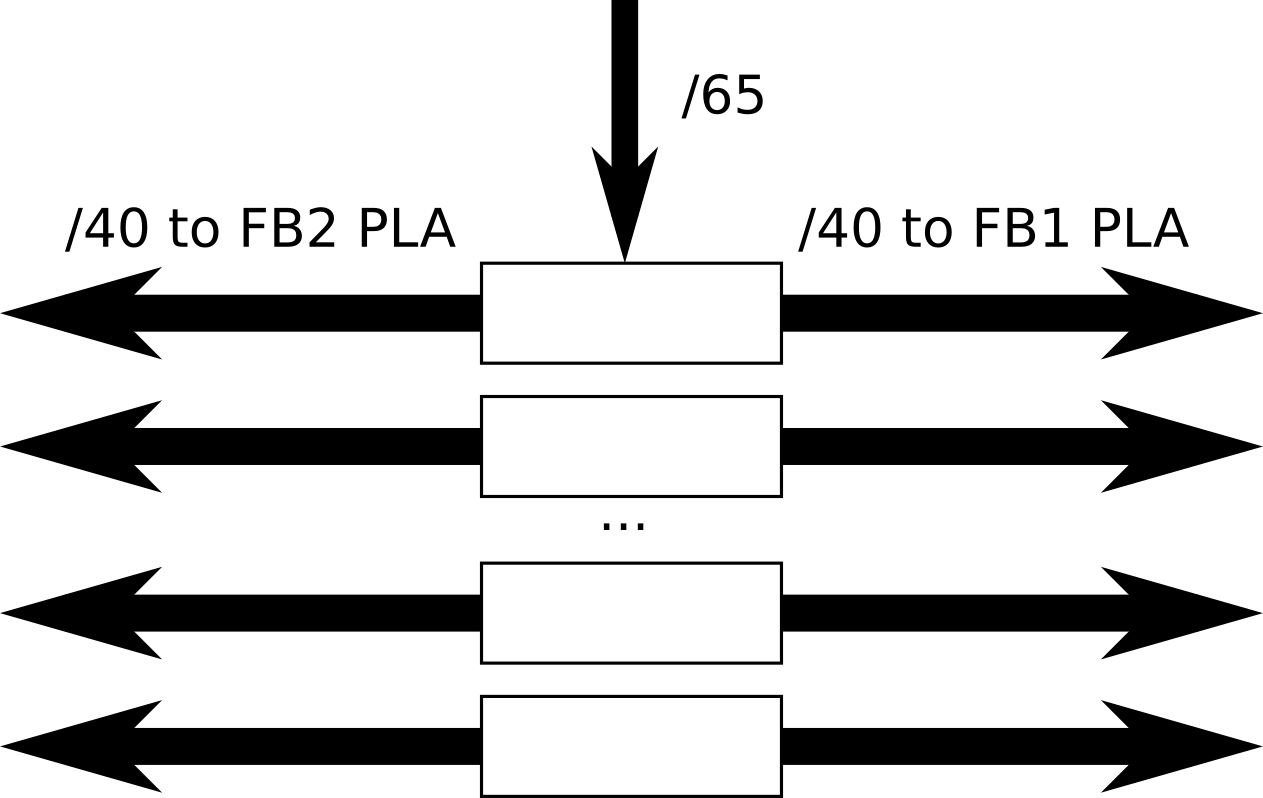
\includegraphics[scale=1]{xc2c32a-zia-block-only.png}
	\caption{XC2C32A ZIA high-level structure}
	\label{xc2c32a-zia-block-only}
\end{figure}

The basic structure of one ZIA cell is a multi-level dual-rooted tree of muxes (Fig. ~\ref {xc2c32a-zia-tree}). At 
the widest level the input data bus is grouped into sets of 11 wires; each group is reduced to one signal by a 
mask-programmed mux (filled). The settings of these mask-programmed muxes are different for each row in the ZIA 
block and also vary between device densities, however each ZIA block in a given device will have the same settings. 
The settings for these muxes in the XC2C32A were recovered by scanning electron microscopy of a delayered die and 
are reproduced in the appendix; settings for other device densities are not yet known.

\begin{figure}[h]
	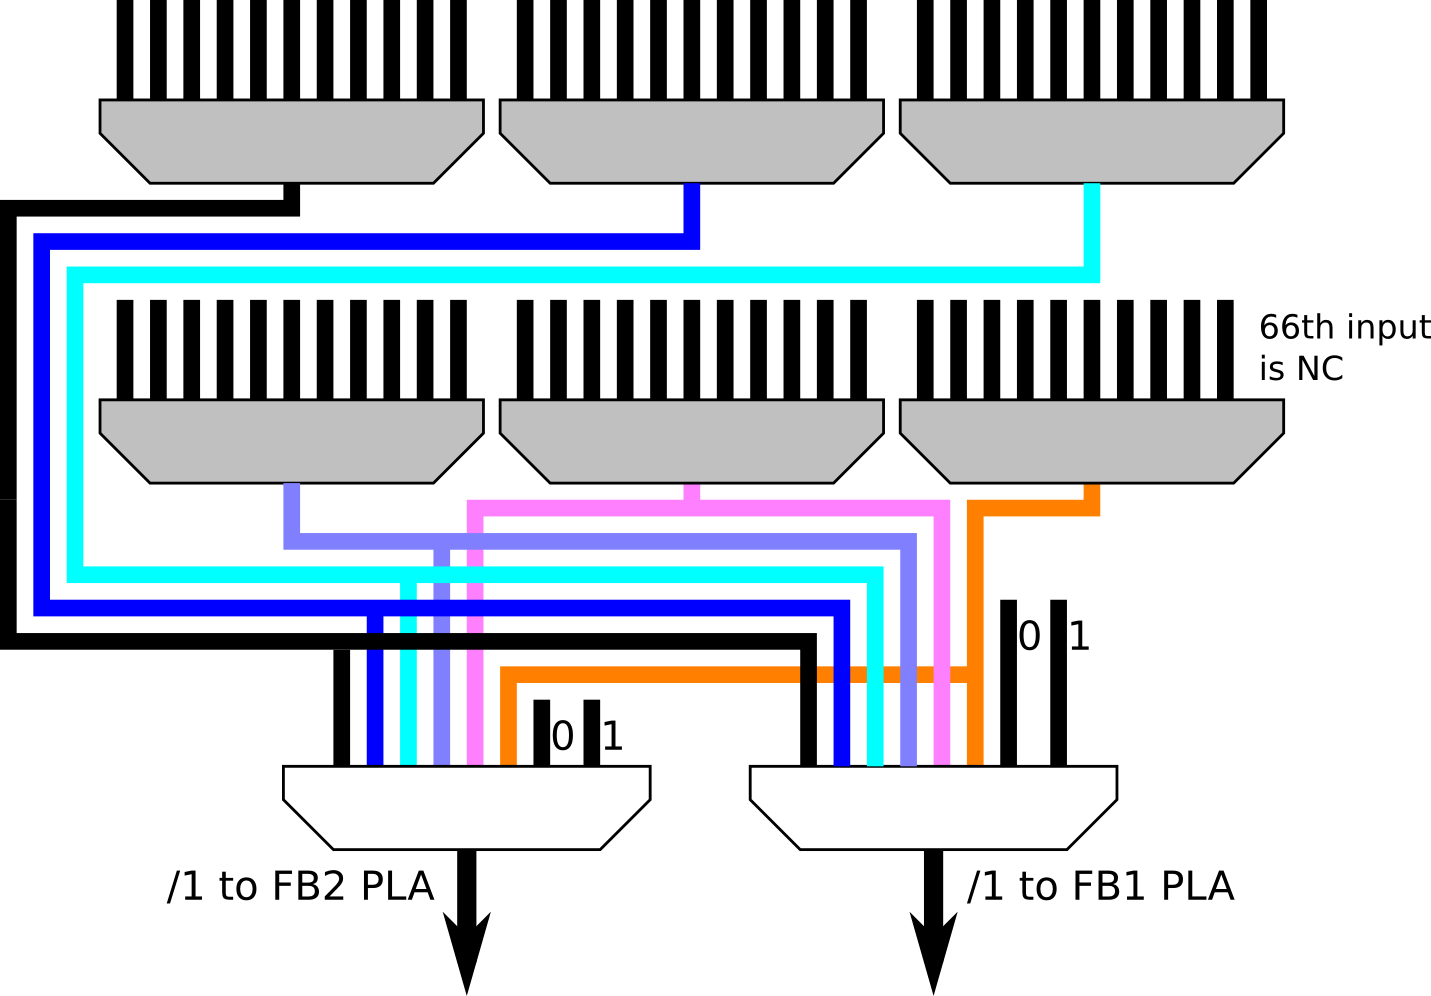
\includegraphics[scale=1]{xc2c32a-zia-tree.png}
	\caption{XC2C32A ZIA tree structure}
	\label{xc2c32a-zia-tree}
\end{figure}

At this point, the reduced signal bus is fed into the next level of the tree, which consists of programmable muxes 
(un-filled). This level, and any subsequent ones, are replicated twice to yield two partially independent roots. In 
other words, while any given ZIA row can only pick from 1/11 of the signals on the global data bus, the left- and 
right-feeding outputs may be chosen fully independently from the reduced data bus. In physical layout the left- and 
right-feeding muxes are stacked vertically; the left-feeding channel is located near the center side of the row 
while the right-feeding channel is on the outer side.

The XC2C32A has only one level of programmable muxing, controlled by eight one-hot bits: each ZIA output may be 
connected to Vdd, Vss, or one of the six inputs from the reduced bus.

The mux trees for the larger devices have not been studied in detail however preliminary inspection of the XC2C256 
suggests a 3-level tree: 11 mask-programmed muxes reducing 440 signals down to 40, six programmable muxes reducing 
these down to six, then one programmable mux to give a final output. The final mux is presumably identical (or 
nearly so) to those in the XC2C32A, with one more intermediate level of programmable muxing which includes pass 
transistors but no pull-high / pull-low capability.

\FloatBarrier
\section{PLA}

\subsection{AND array}

\subsection{OR array}

\section{Macrocells}

\section{I/O blocks}

\section{Flash}

\subsection{Programming}

\subsubsection{Introduction}

Loading a bitstream onto a CoolRunner-II device can be done in two ways: writing to Flash or SRAM. This section 
only covers writing to Flash. The configuration algorithm is described fairly well by Xilinx in \cite{progspec} 
however some details of the actual bitstream structure are glossed over.

\subsubsection{Device enumeration}

The first step is, of course, to verify that a functioning JTAG adapter is connected and that there is a board 
with a valid scan chain plugged into it. The procedure for performing this should be described by your JTAG API.
The remainder of this section assumes that scan operations are being performed on a single-device chain 
consisting solely of the CPLD of interest, if multiple devices are present in the chain appropriate padding bits 
should be inserted.

Once the chain has been enumerated, scan the IDCODE instruction and read 32 bits of data, which should match the 
known ID code of the CPLD of interest. The ID code consists of several bitfields, as described below:

\begin{itemize}
\item 31:28 = stepping number
\item 27:25 = architecture (always 3'h3)
\item 24:16 = device ID
\item 15 = voltage (always 1)
\item 14:12 = package (device dependent)
\item 11:1 = JEDEC vendor ID for Xilinx (11'h49)
\item 0	= padding for IEEE 1149 (always 1'h1)
\end{itemize}

The device IDs are:
\begin{itemize}
\item XC2C32 = 9'h01
\item XC2C32A = 9'h21
\item XC2C64 = 9'h05
\item XC2C64A = 9'h25
\item XC2C128 = 9'h30
\item XC2C256 = 9'h14
\item XC2C384 = 9'h15
\item XC2C512 = 9'h17
\end{itemize}

CoolRunner-II is unique among Xilinx device families in that the device's package is encoded in the JTAG ID code.
(The exact means by which the die is told what package it lives in is unknown as of this writing.) 

The package code is only three bits long and CoolRunner-II devices come in at least ten possible packages, so the 
package code bits do not have uniform meaning across device densities.

\begin{longtabu} to \linewidth {|l|l|l|l|l|l|l|l|l|}
\hline
{\bf Device} & {\bf 0} & {\bf 1} & {\bf 2} & {\bf 3} & {\bf 4} & {\bf 5} & {\bf 6} & {\bf 7} \\
\hline
XC2C32[A] & & QFG32 & & CPG56 & VQG44 & & & \\
\hline
XC2C64[A] & & QFG48 & & CPG132 & VQG100 & CPG56 & VQG44 & \\
\hline
XC2C128 & & & VQG100 & CPG132 & TQG144 & & FTG256 & \\
\hline
XC2C256 & & & VQG100 & CPG132 & TQG144 & PQG208 & FTG256 & \\
\hline
XC2C384 & & & FGG324 & & TQG144 & PQG208 & & FTG256 \\
\hline
XC2C512 & & & FGG324 & & PQG208 & & FTG256 & \\
\hline
\end{longtabu}

\subsubsection{Erasing}

Before a device can be programmed, it must be erased. This sets all of the flash cells to the ``1" state. The 
device architecture ensures that this state is safe and will not lead to bus fights or unwanted behavior.

The erase procedure (see \cite{progspec}) is:
\begin{itemize}
\item Reset the TAP
\item Shift in the ISC\_ENABLE instruction (8'he8)
\item Wait 800 $\mu s$ for device to enter ISC mode
\item Shift in the ISC\_ERASE instruction (8'hed)
\item Wait 100 ms for erase to complete
\item Shift in the ISC\_INIT instruction (8'hF0) to discharge HV
\item Wait 20 $\mu s$ for charge pump to drain
\item Shift in the ISC\_INIT instruction again to boot the CPLD
\item Shift 8'h00 into the DR to cause an ISP\_INIT pulse
\item Wait 800 $\mu s$ for device to initialize
\item Shift in the ISC\_DISABLE (8'hC0) instruction to leave ISC mode
\item Shift in the BYPASS instruction (8'hff) to return the TAP to the idle state
\item (optional) Use the readback procedure (described in the next section) to verify that the device is blank.
\end{itemize}

TODO: Discuss/test data remanence for readback

\subsubsection{Programming}

The configuration bits as actually loaded into the device are structured physically, not logically. 

\subsubsection{Verification}

\subsection{Physical bitstream structure}

The basic element of a CoolRunner-II device at the bitstream level is two function blocks paired back-to-back, 
as shown in Fig. TODO. Individual configuration rows run left-to-right across the block and addresses increase 
from top to bottom.

From left to right in a single configuration row we have data for the left-hand FB's macrocells, the left-hand 
FB PLA, the ZIA (from both FBs, interleaved), the right-hand FB PLA, and the right-hand FB's macrocells. 
Configuration bits for the right-hand FB PLA and macrocells are mirrored horizontally with respect to the left.

TODO: Figure

\subsection{Boot process}

\subsection{Security}

\pagebreak
\section{Appendix A: ZIA ROM mux settings}

\subsection{XC2C32A}

Each mux in the ZIA is configured by eight status bits ZCFG[7:0]. Note that, while all bits are one-hot coded, 
ZCFG[7] is active-high and the remainder are active-low. This was presumably done so that the value 8'b11111111 
(blank device) would pull the ZIA output to a constant ``1" rather than floating. The bits are coded as follows:
\begin{itemize}
\item ZCFG[7]: set high to output constant ``1". Must be held low if any other mux output is used to avoid bus fights.
\item ZCFG[6]: set low to output constant ``0".
\item ZCFG[5:0]: set one bit low to output the corresponding one of MUXIN[5:0].
\end{itemize}

The XC2C32A ZIA has a total of 65 inputs, structured as follows. The physical die layout has the signals ordered with 
ZIABUS[64] at left and ZIABUS[0] at right.

\begin{itemize}
\item ZIABUS[15:0] = FB1\_IBUF[15:0]
\item ZIABUS[16] = dedicated input pin
\item ZIABUS[32:17] = FB2\_IBUF[15:0]
\item ZIABUS[48:33] = FB1\_FF[15:0]
\item ZIABUS[64:49] = FB2\_FF[15:0]
\end{itemize}

For example, ZCFG = 8'b11111111 sets the output of the row to 1 since ZCFG[7] is asserted and ZCFG[6:0] are 
deasserted. ZCFG = 8'b01111110 in row 4 sets the output of the row to FB4\_IBUF[4] since ZCFG[0] is asserted and 
ZCFG[0] for row 4 is ZIABUS[4] / FB4\_IBUF[4]. ZCFG = 8'b00111111 sets the output of the row to 0 since ZCFG[6] is 
asserted. (It is interesting to note that the Xilinx toolchain does not appear to ever produce bitstreams that assert 
ZCFG[6]. The function of this bit was only discovered from full reverse engineering of the silicon.)

\pagebreak
\newgeometry{margin=1.5in}
\begin{landscape}
Each column in the table represents one of the six possible signal inputs MUXIN[5:0] to the final mux. For brevity the 
implied ZIABUS[] is omitted, so 27/FB2\_IBUF[10] is written instead of ZIABUS[27]/FB2\_IBUF[10].

\begin{longtabu} to \linewidth {|l|X|X|X|X|X|X|}
\hline
{\bf Row} & {\bf ZCFG[0]} & {\bf ZCFG[1]} & {\bf ZCFG[2]} & {\bf ZCFG[3]} & {\bf ZCFG[4]} & {\bf ZCFG[5]} \\
\hline
0   & 0/FB1\_IBUF[0]  & 10/FB1\_IBUF[10]  & 22/FB2\_IBUF[5]  & 34/FB1\_FF[1]    & 46/FB1\_FF[13] & 58/FB2\_FF[9] \\
\hline
1   & 1/FB1\_IBUF[1]  & 11/FB1\_IBUF[11]  & 23/FB2\_IBUF[6]  & 41/FB1\_FF[8]    & 48/FB1\_FF[15] & 61/FB2\_FF[12] \\
\hline
2   & 2/FB1\_IBUF[2]  & 12/FB1\_IBUF[12]  & 30/FB2\_IBUF[13] & 35/FB1\_FF[2]    & 53/FB2\_FF[4]  & 60/FB2\_FF[11] \\
\hline
3   & 3/FB1\_IBUF[3]  & 13/FB1\_IBUF[13]  & 26/FB2\_IBUF[9] & 42/FB1\_FF[9]   & 47/FB1\_FF[14] & 55/FB2\_FF[6]  \\
\hline
4   & 4/FB1\_IBUF[4]  & 14/FB1\_IBUF[14]  & 28/FB2\_IBUF[11] & 38/FB1\_FF[5]    & 44/FB1\_FF[11] & 59/FB2\_FF[10] \\
\hline
5   & 5/FB1\_IBUF[5]  & 15/FB1\_IBUF[15]  & 31/FB2\_IBUF[14] & 40/FB1\_FF[7]    & 50/FB2\_FF[1]  & 56/FB2\_FF[7]  \\
\hline
6   & 6/FB1\_IBUF[6]  & 16/Dedicated in & 21/FB2\_IBUF[4]  & 33/FB1\_FF[0]    & 52/FB2\_FF[3]  & 62/FB2\_FF[13] \\
\hline
7   & 7/FB1\_IBUF[7]  & 17/FB2\_IBUF[0]   & 27/FB2\_IBUF[10] & 32/FB2\_IBUF[15] & 45/FB1\_FF[12] & 64/FB2\_FF[15] \\
\hline
8   & 8/FB1\_IBUF[8]  & 18/FB2\_IBUF[1]   & 25/FB2\_IBUF[8]  & 39/FB1\_FF[6]    & 43/FB1\_FF[10] & 57/FB2\_FF[8]  \\
\hline
9   & 9/FB1\_IBUF[9] & 19/FB2\_IBUF[2]   & 24/FB2\_IBUF[7]  & 37/FB1\_FF[4]    & 51/FB2\_FF[2]  & 54/FB2\_FF[5]  \\
\hline
10  & 7/FB1\_IBUF[7]  & 20/FB2\_IBUF[3]   & 29/FB2\_IBUF[12] & 36/FB1\_FF[3]    & 49/FB2\_FF[0]  & 63/FB2\_FF[14] \\
\hline
11  & 0/FB1\_IBUF[0]  & 11/FB1\_IBUF[11]  & 23/FB2\_IBUF[6]  & 35/FB1\_FF[2]    & 47/FB1\_FF[14] & 59/FB2\_FF[10] \\
\hline
12  & 1/FB1\_IBUF[1]  & 12/FB1\_IBUF[12]  & 30/FB2\_IBUF[13] & 37/FB1\_FF[4]    & 50/FB2\_FF[1]  & 64/FB2\_FF[15] \\
\hline
13  & 2/FB1\_IBUF[2]  & 19/FB2\_IBUF[2]   & 24/FB2\_IBUF[7]  & 42/FB1\_FF[9]   & 49/FB2\_FF[0]  & 62/FB2\_FF[13] \\
\hline
14  & 3/FB1\_IBUF[3]  & 15/FB1\_IBUF[15]  & 31/FB2\_IBUF[14] & 36/FB1\_FF[3]    & 44/FB1\_FF[11] & 61/FB2\_FF[12] \\
\hline
15  & 4/FB1\_IBUF[4]  & 17/FB2\_IBUF[0]   & 27/FB2\_IBUF[10] & 33/FB1\_FF[0]    & 48/FB1\_FF[15] & 56/FB2\_FF[7]  \\
\hline
16  & 5/FB1\_IBUF[5]  & 20/FB2\_IBUF[3]   & 29/FB2\_IBUF[12] & 39/FB1\_FF[6]    & 45/FB1\_FF[12] & 60/FB2\_FF[11] \\
\hline
17  & 6/FB1\_IBUF[6]  & 10/FB1\_IBUF[10]  & 22/FB2\_IBUF[5]  & 41/FB1\_FF[8]    & 51/FB2\_FF[2]  & 57/FB2\_FF[8]  \\
\hline
18  & 7/FB1\_IBUF[7]  & 16/Dedicated in & 21/FB2\_IBUF[4]  & 34/FB1\_FF[1]    & 53/FB2\_FF[4]  & 63/FB2\_FF[14] \\
\hline
19  & 8/FB1\_IBUF[8]  & 14/FB1\_IBUF[14]  & 28/FB2\_IBUF[11] & 32/FB2\_IBUF[15] & 46/FB1\_FF[13] & 55/FB2\_FF[6]  \\
\hline
20  & 9/FB1\_IBUF[9] & 13/FB1\_IBUF[13]  & 26/FB2\_IBUF[9] & 40/FB1\_FF[7]    & 43/FB1\_FF[10] & 58/FB2\_FF[9] \\
\hline
21  & 8/FB1\_IBUF[8]  & 18/FB2\_IBUF[1]   & 25/FB2\_IBUF[8]  & 38/FB1\_FF[5]    & 52/FB2\_FF[3]  & 54/FB2\_FF[5]  \\
\hline
22  & 0/FB1\_IBUF[0]  & 12/FB1\_IBUF[12]  & 24/FB2\_IBUF[7]  & 36/FB1\_FF[3]    & 48/FB1\_FF[15] & 60/FB2\_FF[11] \\
\hline
23  & 1/FB1\_IBUF[1]  & 19/FB2\_IBUF[2]   & 26/FB2\_IBUF[9] & 39/FB1\_FF[6]    & 53/FB2\_FF[4]  & 54/FB2\_FF[5]  \\
\hline
24  & 2/FB1\_IBUF[2]  & 13/FB1\_IBUF[13]  & 31/FB2\_IBUF[14] & 38/FB1\_FF[5]    & 51/FB2\_FF[2]  & 55/FB2\_FF[6]  \\
\hline
25  & 3/FB1\_IBUF[3]  & 20/FB2\_IBUF[3]   & 25/FB2\_IBUF[8]  & 33/FB1\_FF[0]    & 50/FB2\_FF[1]  & 63/FB2\_FF[14] \\
\hline
26  & 4/FB1\_IBUF[4]  & 16/Dedicated in & 22/FB2\_IBUF[5]  & 37/FB1\_FF[4]    & 45/FB1\_FF[12] & 62/FB2\_FF[13] \\
\hline
27  & 5/FB1\_IBUF[5]  & 18/FB2\_IBUF[1]   & 28/FB2\_IBUF[11] & 34/FB1\_FF[1]    & 49/FB2\_FF[0]  & 57/FB2\_FF[8]  \\
\hline
28  & 6/FB1\_IBUF[6]  & 11/FB1\_IBUF[11]  & 30/FB2\_IBUF[13] & 40/FB1\_FF[7]    & 46/FB1\_FF[13] & 61/FB2\_FF[12] \\
\hline
29  & 7/FB1\_IBUF[7]  & 10/FB1\_IBUF[10]  & 23/FB2\_IBUF[6]  & 42/FB1\_FF[9]   & 52/FB2\_FF[3]  & 58/FB2\_FF[9] \\
\hline
30  & 8/FB1\_IBUF[8]  & 17/FB2\_IBUF[0]   & 21/FB2\_IBUF[4]  & 35/FB1\_FF[2]    & 44/FB1\_FF[11] & 64/FB2\_FF[15] \\
\hline
31  & 9/FB1\_IBUF[9] & 15/FB1\_IBUF[15]  & 29/FB2\_IBUF[12] & 32/FB2\_IBUF[15] & 47/FB1\_FF[14] & 56/FB2\_FF[7]  \\
\hline
32  & 9/FB1\_IBUF[9] & 14/FB1\_IBUF[14]  & 27/FB2\_IBUF[10] & 41/FB1\_FF[8]    & 43/FB1\_FF[10] & 59/FB2\_FF[10] \\
\hline
33  & 0/FB1\_IBUF[0]  & 13/FB1\_IBUF[13]  & 25/FB2\_IBUF[8]  & 37/FB1\_FF[4]    & 49/FB2\_FF[0]  & 61/FB2\_FF[12] \\
\hline
34  & 1/FB1\_IBUF[1]  & 15/FB1\_IBUF[15]  & 28/FB2\_IBUF[11] & 42/FB1\_FF[9]   & 43/FB1\_FF[10] & 60/FB2\_FF[11] \\
\hline
35  & 2/FB1\_IBUF[2]  & 20/FB2\_IBUF[3]   & 27/FB2\_IBUF[10] & 40/FB1\_FF[7]    & 44/FB1\_FF[11] & 54/FB2\_FF[5]  \\
\hline
36  & 3/FB1\_IBUF[3]  & 14/FB1\_IBUF[14]  & 22/FB2\_IBUF[5]  & 39/FB1\_FF[6]    & 52/FB2\_FF[3]  & 56/FB2\_FF[7]  \\
\hline
37  & 4/FB1\_IBUF[4]  & 11/FB1\_IBUF[11]  & 26/FB2\_IBUF[9] & 34/FB1\_FF[1]    & 51/FB2\_FF[2]  & 64/FB2\_FF[15] \\
\hline
38  & 5/FB1\_IBUF[5]  & 17/FB2\_IBUF[0]   & 23/FB2\_IBUF[6]  & 38/FB1\_FF[5]    & 46/FB1\_FF[13] & 63/FB2\_FF[14] \\
\hline
39  & 6/FB1\_IBUF[6]  & 19/FB2\_IBUF[2]   & 29/FB2\_IBUF[12] & 35/FB1\_FF[2]    & 50/FB2\_FF[1]  & 58/FB2\_FF[9] \\
\hline
\end{longtabu}
\end{landscape}
\restoregeometry

\pagebreak
\section{Appendix B: Virtual-to-ISC address mapping}

\pagebreak
\bibliography{not-datasheet}{}
\bibliographystyle{acm}

\end{document}
